% Options for packages loaded elsewhere
\PassOptionsToPackage{unicode}{hyperref}
\PassOptionsToPackage{hyphens}{url}
%
\documentclass[
]{article}
\usepackage{lmodern}
\usepackage{amssymb,amsmath}
\usepackage{ifxetex,ifluatex}
\ifnum 0\ifxetex 1\fi\ifluatex 1\fi=0 % if pdftex
  \usepackage[T1]{fontenc}
  \usepackage[utf8]{inputenc}
  \usepackage{textcomp} % provide euro and other symbols
\else % if luatex or xetex
  \usepackage{unicode-math}
  \defaultfontfeatures{Scale=MatchLowercase}
  \defaultfontfeatures[\rmfamily]{Ligatures=TeX,Scale=1}
\fi
% Use upquote if available, for straight quotes in verbatim environments
\IfFileExists{upquote.sty}{\usepackage{upquote}}{}
\IfFileExists{microtype.sty}{% use microtype if available
  \usepackage[]{microtype}
  \UseMicrotypeSet[protrusion]{basicmath} % disable protrusion for tt fonts
}{}
\makeatletter
\@ifundefined{KOMAClassName}{% if non-KOMA class
  \IfFileExists{parskip.sty}{%
    \usepackage{parskip}
  }{% else
    \setlength{\parindent}{0pt}
    \setlength{\parskip}{6pt plus 2pt minus 1pt}}
}{% if KOMA class
  \KOMAoptions{parskip=half}}
\makeatother
\usepackage{xcolor}
\IfFileExists{xurl.sty}{\usepackage{xurl}}{} % add URL line breaks if available
\IfFileExists{bookmark.sty}{\usepackage{bookmark}}{\usepackage{hyperref}}
\hypersetup{
  pdftitle={Reason Theme/Graphics},
  pdfauthor={Anil},
  hidelinks,
  pdfcreator={LaTeX via pandoc}}
\urlstyle{same} % disable monospaced font for URLs
\usepackage[margin=1in]{geometry}
\usepackage{color}
\usepackage{fancyvrb}
\newcommand{\VerbBar}{|}
\newcommand{\VERB}{\Verb[commandchars=\\\{\}]}
\DefineVerbatimEnvironment{Highlighting}{Verbatim}{commandchars=\\\{\}}
% Add ',fontsize=\small' for more characters per line
\usepackage{framed}
\definecolor{shadecolor}{RGB}{248,248,248}
\newenvironment{Shaded}{\begin{snugshade}}{\end{snugshade}}
\newcommand{\AlertTok}[1]{\textcolor[rgb]{0.94,0.16,0.16}{#1}}
\newcommand{\AnnotationTok}[1]{\textcolor[rgb]{0.56,0.35,0.01}{\textbf{\textit{#1}}}}
\newcommand{\AttributeTok}[1]{\textcolor[rgb]{0.77,0.63,0.00}{#1}}
\newcommand{\BaseNTok}[1]{\textcolor[rgb]{0.00,0.00,0.81}{#1}}
\newcommand{\BuiltInTok}[1]{#1}
\newcommand{\CharTok}[1]{\textcolor[rgb]{0.31,0.60,0.02}{#1}}
\newcommand{\CommentTok}[1]{\textcolor[rgb]{0.56,0.35,0.01}{\textit{#1}}}
\newcommand{\CommentVarTok}[1]{\textcolor[rgb]{0.56,0.35,0.01}{\textbf{\textit{#1}}}}
\newcommand{\ConstantTok}[1]{\textcolor[rgb]{0.00,0.00,0.00}{#1}}
\newcommand{\ControlFlowTok}[1]{\textcolor[rgb]{0.13,0.29,0.53}{\textbf{#1}}}
\newcommand{\DataTypeTok}[1]{\textcolor[rgb]{0.13,0.29,0.53}{#1}}
\newcommand{\DecValTok}[1]{\textcolor[rgb]{0.00,0.00,0.81}{#1}}
\newcommand{\DocumentationTok}[1]{\textcolor[rgb]{0.56,0.35,0.01}{\textbf{\textit{#1}}}}
\newcommand{\ErrorTok}[1]{\textcolor[rgb]{0.64,0.00,0.00}{\textbf{#1}}}
\newcommand{\ExtensionTok}[1]{#1}
\newcommand{\FloatTok}[1]{\textcolor[rgb]{0.00,0.00,0.81}{#1}}
\newcommand{\FunctionTok}[1]{\textcolor[rgb]{0.00,0.00,0.00}{#1}}
\newcommand{\ImportTok}[1]{#1}
\newcommand{\InformationTok}[1]{\textcolor[rgb]{0.56,0.35,0.01}{\textbf{\textit{#1}}}}
\newcommand{\KeywordTok}[1]{\textcolor[rgb]{0.13,0.29,0.53}{\textbf{#1}}}
\newcommand{\NormalTok}[1]{#1}
\newcommand{\OperatorTok}[1]{\textcolor[rgb]{0.81,0.36,0.00}{\textbf{#1}}}
\newcommand{\OtherTok}[1]{\textcolor[rgb]{0.56,0.35,0.01}{#1}}
\newcommand{\PreprocessorTok}[1]{\textcolor[rgb]{0.56,0.35,0.01}{\textit{#1}}}
\newcommand{\RegionMarkerTok}[1]{#1}
\newcommand{\SpecialCharTok}[1]{\textcolor[rgb]{0.00,0.00,0.00}{#1}}
\newcommand{\SpecialStringTok}[1]{\textcolor[rgb]{0.31,0.60,0.02}{#1}}
\newcommand{\StringTok}[1]{\textcolor[rgb]{0.31,0.60,0.02}{#1}}
\newcommand{\VariableTok}[1]{\textcolor[rgb]{0.00,0.00,0.00}{#1}}
\newcommand{\VerbatimStringTok}[1]{\textcolor[rgb]{0.31,0.60,0.02}{#1}}
\newcommand{\WarningTok}[1]{\textcolor[rgb]{0.56,0.35,0.01}{\textbf{\textit{#1}}}}
\usepackage{graphicx,grffile}
\makeatletter
\def\maxwidth{\ifdim\Gin@nat@width>\linewidth\linewidth\else\Gin@nat@width\fi}
\def\maxheight{\ifdim\Gin@nat@height>\textheight\textheight\else\Gin@nat@height\fi}
\makeatother
% Scale images if necessary, so that they will not overflow the page
% margins by default, and it is still possible to overwrite the defaults
% using explicit options in \includegraphics[width, height, ...]{}
\setkeys{Gin}{width=\maxwidth,height=\maxheight,keepaspectratio}
% Set default figure placement to htbp
\makeatletter
\def\fps@figure{htbp}
\makeatother
\setlength{\emergencystretch}{3em} % prevent overfull lines
\providecommand{\tightlist}{%
  \setlength{\itemsep}{0pt}\setlength{\parskip}{0pt}}
\setcounter{secnumdepth}{-\maxdimen} % remove section numbering

\title{Reason Theme/Graphics}
\author{Anil}
\date{6/30/2020}

\begin{document}
\maketitle

\hypertarget{r-markdown}{%
\subsection{R Markdown}\label{r-markdown}}

This is an R Markdown document that describes Reason graphics style in
R. Packages: \texttt{pensionviewr} \& \texttt{reasonTheme}

\#\#Defining - Colors - ggplot() themes, labels, and margins

\begin{Shaded}
\begin{Highlighting}[]
\CommentTok{# All images should use web safe colors — this gives us a range of orange and blue}
\CommentTok{# colors that fit with Reason’s branding, as well as reds and greens that we can use to}
\CommentTok{# indicate positive or negative data patterns. The following colors are most suitable:}
\CommentTok{#https://www.rapidtables.com/web/color/Web_Safe.html}

\NormalTok{palette_reason <-}\StringTok{ }\KeywordTok{data.frame}\NormalTok{(}
  \DataTypeTok{Orange =} \StringTok{"#FF6633"}\NormalTok{, }
  \DataTypeTok{Yellow =} \StringTok{"#FFCC33"}\NormalTok{, }
  \DataTypeTok{LightOrange =} \StringTok{"#FF9933"}\NormalTok{,}
  \DataTypeTok{DarkGrey =} \StringTok{"#333333"}\NormalTok{, }
  \DataTypeTok{SpaceGrey =} \StringTok{"#A69FA1"}\NormalTok{,}
  \DataTypeTok{DarkBlue =} \StringTok{"#0066CC"}\NormalTok{,}
  \DataTypeTok{GreyBlue =} \StringTok{"#6699CC"}\NormalTok{, }
  \DataTypeTok{LightBlue =} \StringTok{"#3399CC"}\NormalTok{, }
  \DataTypeTok{Yellow =} \StringTok{"#FFCC33"}\NormalTok{, }
  \DataTypeTok{LightBlue =} \StringTok{"#66B2FF"}\NormalTok{, }
  \DataTypeTok{SatBlue =} \StringTok{"#3366CC"}\NormalTok{, }
  \DataTypeTok{Green =} \StringTok{"#669900"}\NormalTok{,}
  \DataTypeTok{LightGreen =} \StringTok{"#00CC66"}\NormalTok{,}
  \DataTypeTok{Red =} \StringTok{"#CC0000"}\NormalTok{,}
  \DataTypeTok{LightRed =} \StringTok{"#FF0000"}\NormalTok{)}

\CommentTok{##Convert color code to RedGreenBlue palette (with rgb())}
\NormalTok{rgb1 <-}\StringTok{ }\KeywordTok{col2rgb}\NormalTok{(palette_reason}\OperatorTok{$}\NormalTok{SatBlue, }\DataTypeTok{alpha =} \OtherTok{FALSE}\NormalTok{)}\OperatorTok{/}\DecValTok{255}
\NormalTok{rgb1}
\end{Highlighting}
\end{Shaded}

\begin{verbatim}
##       [,1]
## red    0.2
## green  0.4
## blue   0.8
\end{verbatim}

\begin{Shaded}
\begin{Highlighting}[]
\KeywordTok{rownames}\NormalTok{(rgb1) <-}\StringTok{ }\KeywordTok{c}\NormalTok{(}\StringTok{"red"}\NormalTok{, }\StringTok{"green"}\NormalTok{, }\StringTok{"blue"}\NormalTok{)}
\NormalTok{ColorName <-}\StringTok{ }\KeywordTok{rgb}\NormalTok{(rgb1[}\DecValTok{1}\NormalTok{],rgb1[}\DecValTok{2}\NormalTok{],rgb1[}\DecValTok{3}\NormalTok{])}
\NormalTok{ColorName}
\end{Highlighting}
\end{Shaded}

\begin{verbatim}
## [1] "#3366CC"
\end{verbatim}

\begin{Shaded}
\begin{Highlighting}[]
\CommentTok{#Customize color code}
\NormalTok{ColorName2 <-}\StringTok{ }\KeywordTok{rgb}\NormalTok{(}\FloatTok{0.1}\NormalTok{,}\FloatTok{0.5}\NormalTok{,}\FloatTok{0.8}\NormalTok{)}
\NormalTok{ColorName2}
\end{Highlighting}
\end{Shaded}

\begin{verbatim}
## [1] "#1A80CC"
\end{verbatim}

\begin{Shaded}
\begin{Highlighting}[]
\CommentTok{#######}
\ControlFlowTok{for}\NormalTok{ (i }\ControlFlowTok{in}\NormalTok{ (}\DecValTok{1}\OperatorTok{:}\KeywordTok{length}\NormalTok{(palette_reason)))\{}
\NormalTok{x <-}\StringTok{ }\KeywordTok{plot}\NormalTok{(}\KeywordTok{c}\NormalTok{(}\DecValTok{5}\NormalTok{, }\DecValTok{10}\NormalTok{), }\KeywordTok{c}\NormalTok{(}\DecValTok{15}\NormalTok{, }\DecValTok{30}\NormalTok{), }\DataTypeTok{type=} \StringTok{"n"}\NormalTok{, }\DataTypeTok{main=}\KeywordTok{c}\NormalTok{(}\KeywordTok{colnames}\NormalTok{(palette_reason[i])), }\DataTypeTok{xlab =} \StringTok{""}\NormalTok{, }
\DataTypeTok{ylab =} \KeywordTok{c}\NormalTok{(}\KeywordTok{as.character}\NormalTok{(palette_reason[}\DecValTok{1}\NormalTok{,i])), }\DataTypeTok{xaxt=}\StringTok{"n"}\NormalTok{, }\DataTypeTok{yaxt=}\StringTok{"n"}\NormalTok{,}\DataTypeTok{cex.lab=}\FloatTok{1.5}\NormalTok{, }\DataTypeTok{cex.main=}\DecValTok{2}\NormalTok{)}
\KeywordTok{rect}\NormalTok{(}\DecValTok{5}\NormalTok{, }\DecValTok{15}\NormalTok{, }\DecValTok{10}\NormalTok{, }\DecValTok{30}\NormalTok{, }\DataTypeTok{col =} \KeywordTok{as.character}\NormalTok{(palette_reason[}\DecValTok{1}\NormalTok{,i]), }\DataTypeTok{border =} \StringTok{"transparent"}\NormalTok{)}
\CommentTok{## Standard Colors for graphics in R}
\NormalTok{\}}
\end{Highlighting}
\end{Shaded}

\includegraphics[width=200px]{ReasonTheme_files/figure-latex/unnamed-chunk-1-1}
\includegraphics[width=200px]{ReasonTheme_files/figure-latex/unnamed-chunk-1-2}
\includegraphics[width=200px]{ReasonTheme_files/figure-latex/unnamed-chunk-1-3}
\includegraphics[width=200px]{ReasonTheme_files/figure-latex/unnamed-chunk-1-4}
\includegraphics[width=200px]{ReasonTheme_files/figure-latex/unnamed-chunk-1-5}
\includegraphics[width=200px]{ReasonTheme_files/figure-latex/unnamed-chunk-1-6}
\includegraphics[width=200px]{ReasonTheme_files/figure-latex/unnamed-chunk-1-7}
\includegraphics[width=200px]{ReasonTheme_files/figure-latex/unnamed-chunk-1-8}
\includegraphics[width=200px]{ReasonTheme_files/figure-latex/unnamed-chunk-1-9}
\includegraphics[width=200px]{ReasonTheme_files/figure-latex/unnamed-chunk-1-10}
\includegraphics[width=200px]{ReasonTheme_files/figure-latex/unnamed-chunk-1-11}
\includegraphics[width=200px]{ReasonTheme_files/figure-latex/unnamed-chunk-1-12}
\includegraphics[width=200px]{ReasonTheme_files/figure-latex/unnamed-chunk-1-13}
\includegraphics[width=200px]{ReasonTheme_files/figure-latex/unnamed-chunk-1-14}
\includegraphics[width=200px]{ReasonTheme_files/figure-latex/unnamed-chunk-1-15}

\hypertarget{standardized-r-parameters}{%
\section{Standardized R parameters:}\label{standardized-r-parameters}}

\hypertarget{base-r-package-ggplot2-main-parts}{%
\subsubsection{Base R package: ggplot2 (main
parts)}\label{base-r-package-ggplot2-main-parts}}

\begin{itemize}
\tightlist
\item
  geometry (ex: line, bar, point, text)
\item
  scale (ex: x-axis, y-axis, color, shape)
\item
  mapping of data to scales (ex: car type maps to the x-axis)
\item
  theme (ex: title font, caption color)
\end{itemize}

\hypertarget{base-font-calibri}{%
\subsubsection{Base Font: ``Calibri''}\label{base-font-calibri}}

\hypertarget{base-font-size-14.0}{%
\subsubsection{Base Font size: 14.0}\label{base-font-size-14.0}}

\hypertarget{base-line-size-0.5}{%
\subsubsection{Base Line size: 0.5}\label{base-line-size-0.5}}

\hypertarget{base-theme-reasontheme}{%
\subsubsection{Base Theme: reasonTheme (}\label{base-theme-reasontheme}}

\begin{verbatim}
 #plot.title (size = base_size * 12 / 8.5, margin = ggplot2::margin(b = 10L))
 #plot.margin (t = half_line,
                              r = base_line_size * 24,
                              b = half_line,
                              l = half_line)
 #axis.title(face = "bold", size = base_size)
 #axis.title.x(margin = ggplot2::margin(t = 8L))
 #axis.title.y(angle = 90L,margin = ggplot2::margin(r = 4L))
 #axis.ticks.length(4L, "pt")
  
                
\end{verbatim}

\hypertarget{what-you-have-to-specify-in-ggplot-after-setting-reason-theme-when-you-graph-somthing-in-r}{%
\subsubsection{What you have to specify in ggplot(), after setting
Reason theme, when you graph somthing in
R:}\label{what-you-have-to-specify-in-ggplot-after-setting-reason-theme-when-you-graph-somthing-in-r}}

\begin{itemize}
\tightlist
\item
  Data to use for the graph (data.frame)
\item
  Y-axis \& X-axis scales (\texttt{ticks\ =\ n})
\item
  Y-axis \& X-axis limits (\texttt{limits\ =\ c(x,y)})
\item
  Colors (\texttt{color\ =} or \texttt{fill\ =}, using colors in
  \texttt{palette\_reason})
\item
  Title (\texttt{ggtitle()})
\end{itemize}

\hypertarget{latest-mountain-of-debt-plot-using-deptplot-from-pensionviewr}{%
\subsection{\texorpdfstring{Latest Mountain of Debt Plot using
deptPlot() from
\texttt{pensionviewr}}{Latest Mountain of Debt Plot using deptPlot() from pensionviewr}}\label{latest-mountain-of-debt-plot-using-deptplot-from-pensionviewr}}

\hypertarget{modified-colors-ending-ticks-year-labels}{%
\subsubsection{Modified colors, ending ticks \& year
labels}\label{modified-colors-ending-ticks-year-labels}}

\begin{figure}
\centering
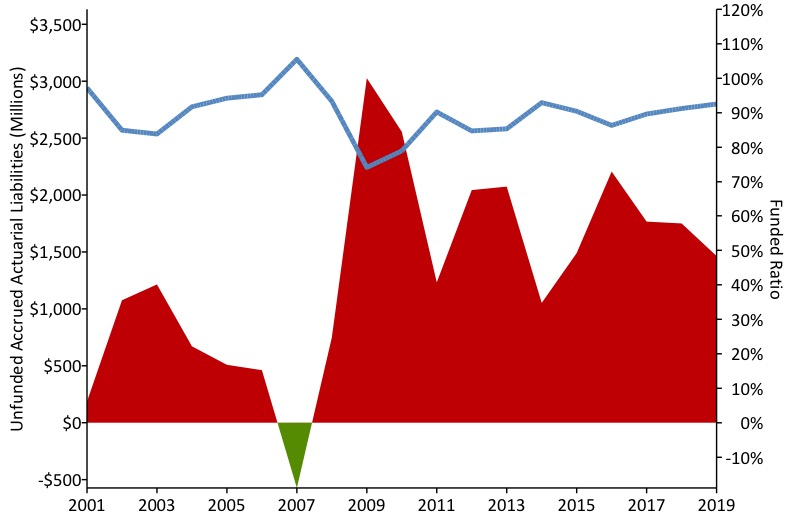
\includegraphics{PERSI.debptPlot2.jpeg}
\caption{Latest Modified Debt Plot - PERSI}
\end{figure}

\hypertarget{original-mountain-of-debt-plot-using-deptplot-from-pensionviewr}{%
\subsection{\texorpdfstring{Original Mountain of Debt Plot using
deptPlot() from
\texttt{pensionviewr}}{Original Mountain of Debt Plot using deptPlot() from pensionviewr}}\label{original-mountain-of-debt-plot-using-deptplot-from-pensionviewr}}

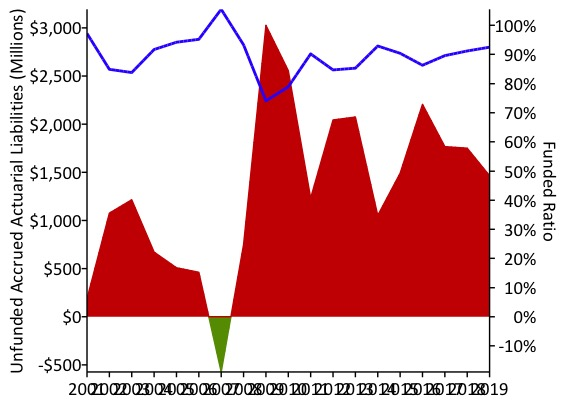
\includegraphics{graphs/DebtPlot.Orig.jpeg} \#\# Modified linePlot()
from \texttt{pensionviewr}(added variables, color palette, and moved
legends) 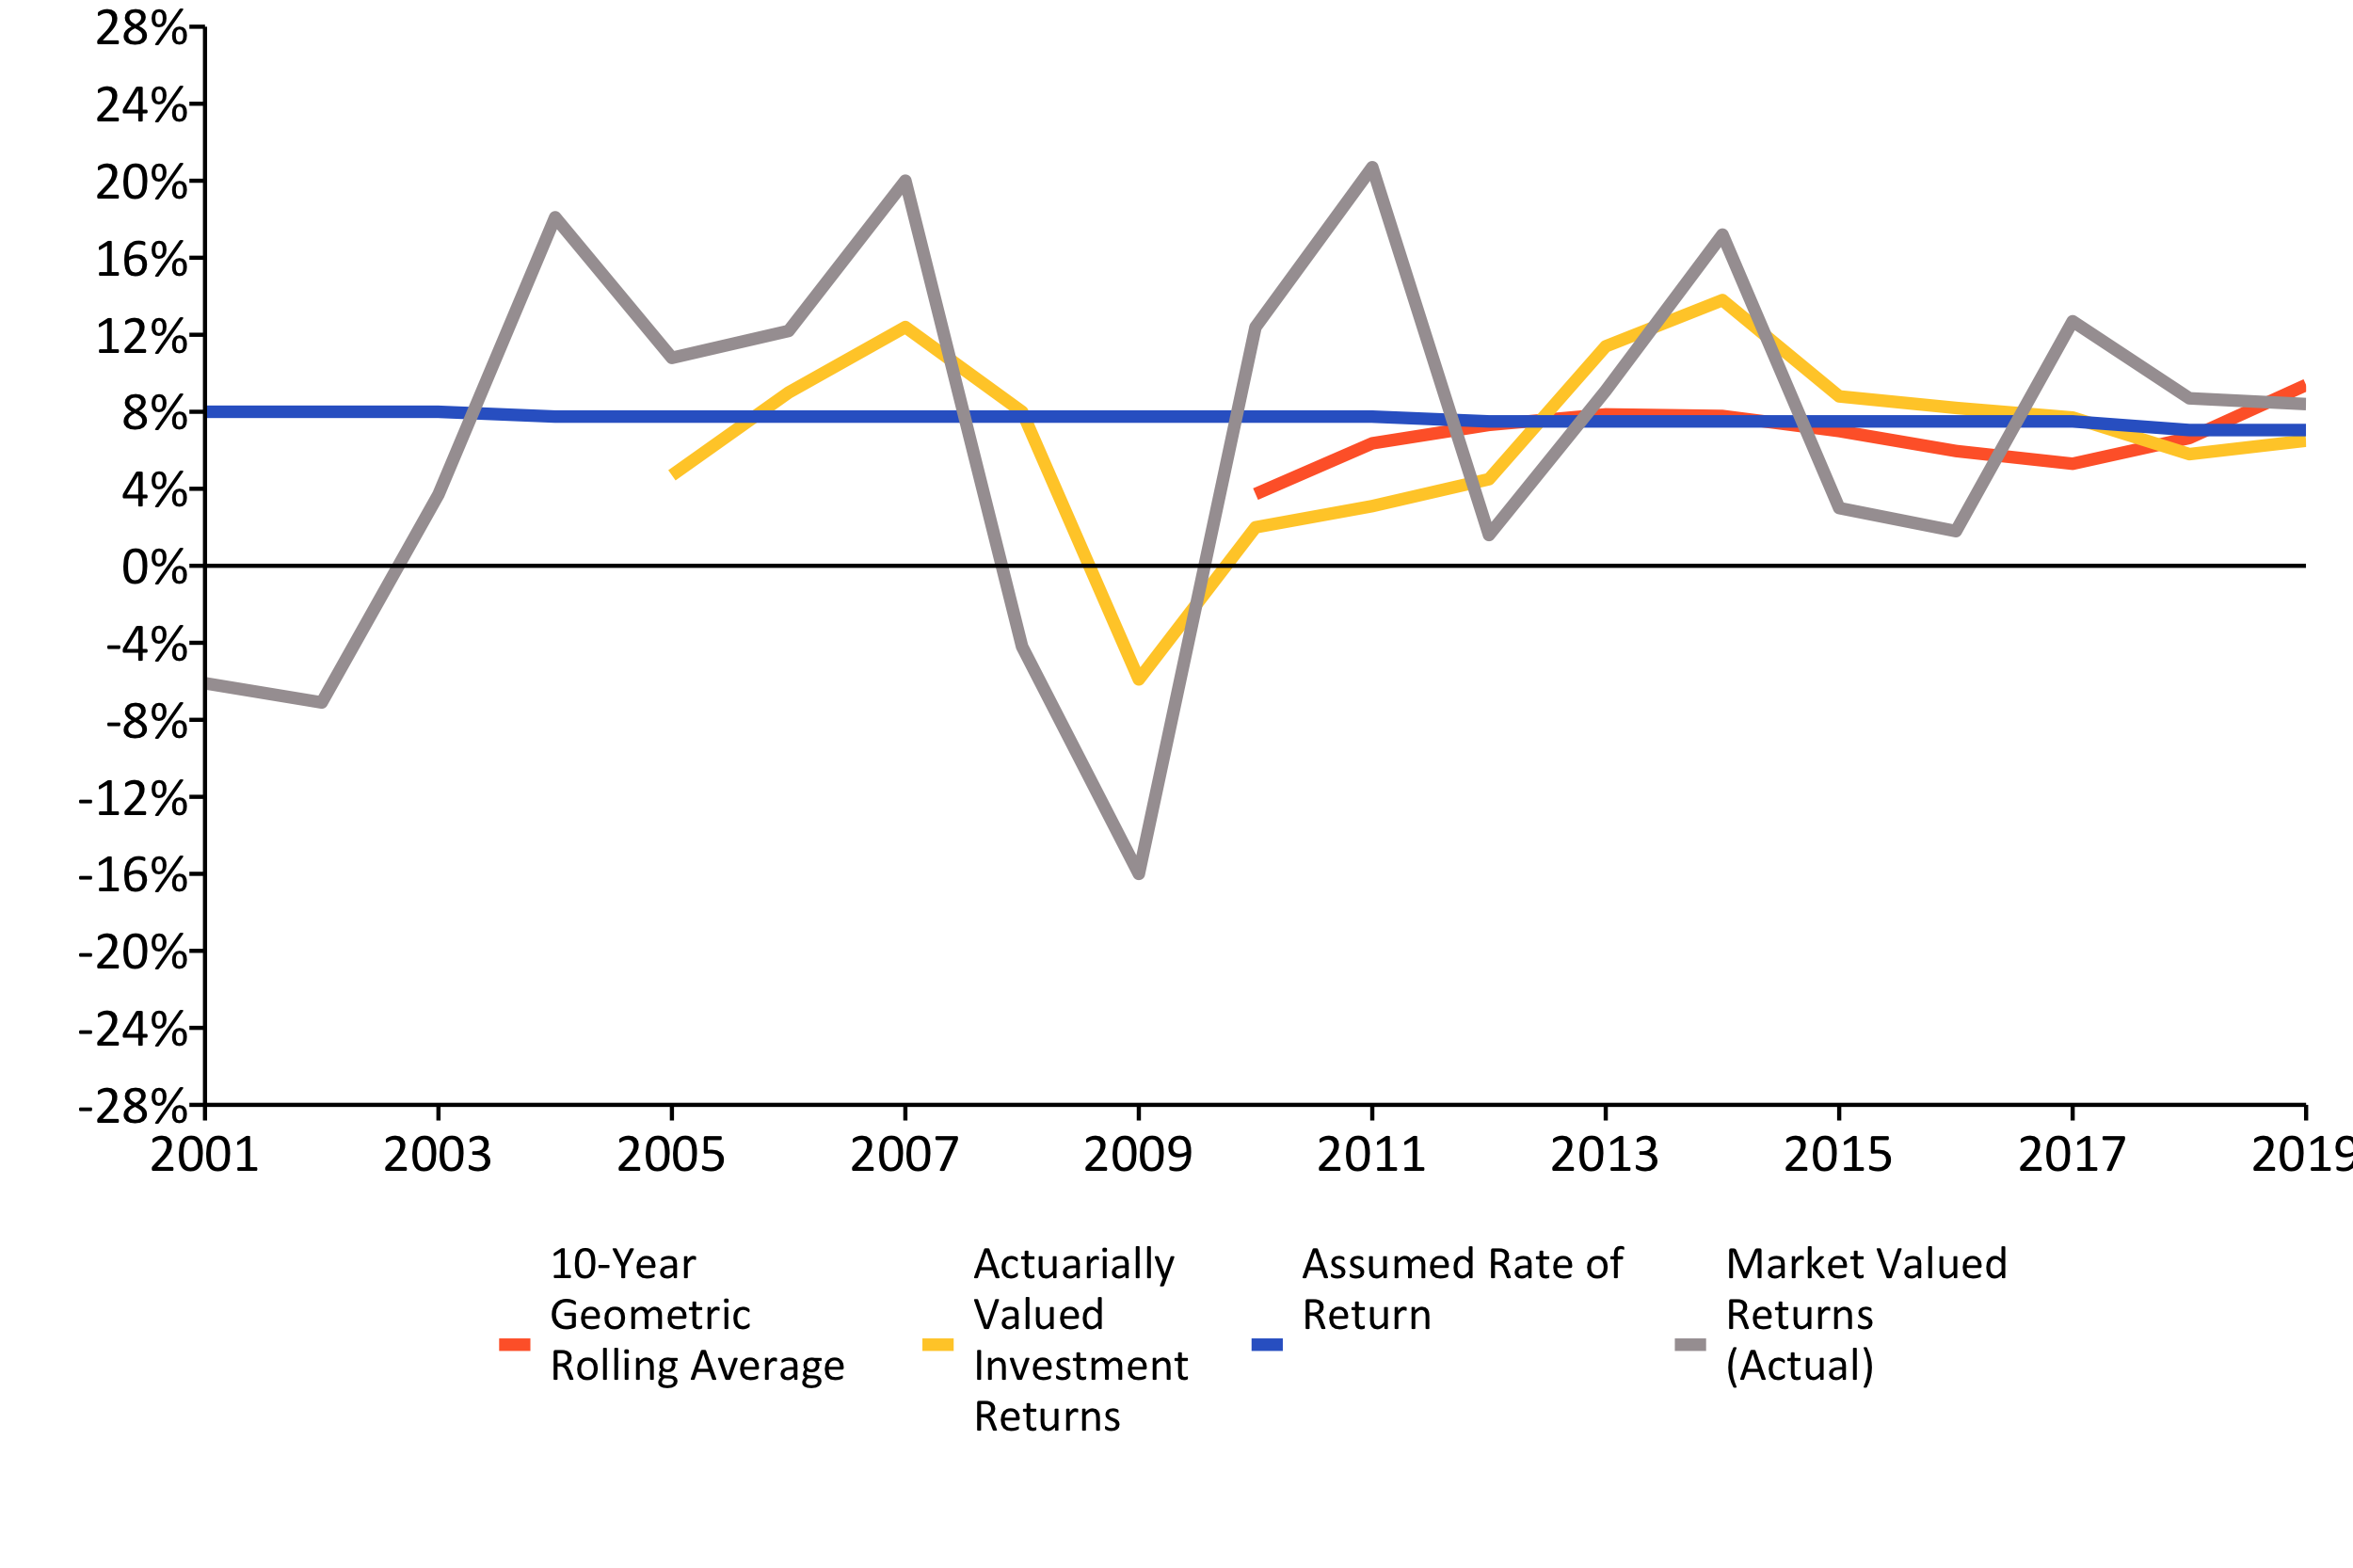
\includegraphics{graphs/Inv.Returns.PERSI.png}

\end{document}
